

%%%%%%%%%%%%%%%%%%%%%%%%%%%%%%%%%%%%%%%%%%%
%\ymignore{
%\begin{leftbar}
% \chapter{Linear Programming Solutions}
% \label{chapter:LP}



An alternative approach to value and policy iteration is the linear programming method. Here the optimal control problem is formulated as a linear program (LP), which can be solved efficiently using standard LP solvers.  
%
In this chapter we will briefly overview the Linear Programming in general and the Linear Program approach for planning in MDPs. We do not attempt in any way to cover the area of linear programming optimization.
There are many excellent books that cover linear programming, for example \cite{Karloff-LP,chvatal1983linear,vanderbei1998linear}. 

%There are two formulations: primal and dual. As this method is less related to learning we will only sketch it briefly.

\section{Background}

%\subsection{Some Background on Linear Programming}
A Linear Program (LP) is an optimization problem that involves
minimizing (or maximizing) a linear objective function subject to
linear constraints. A standard form of an LP is
\begin{equation}\label{eq:LP}
 \textrm{minimize } {b^\top}x,   \quad \textrm{subject to } Ax \ge c,  x \ge 0,
\end{equation}
where $x = {({x_1},{x_2}, \ldots ,{x_n})^\top}$ is a vector of real
variables arranged as a column vector. The set of linear constraints defines a \emph{convex polytope} in $\reals^n$, namely a
closed and convex set $U$ that is the intersection of a finite
number of half-spaces. The set $U$ has a finite number of vertices, which are points that cannot be represented as a convex combination of other points in $U$. If $U$ is bounded, it equals the convex combination of its vertices. It can be seen that an optimal solution (if finite) will be in one of these vertices.

The LP problem has been extensively studied, and many efficient solvers exist. In 1947, Danzig introduced the Simplex algorithm, which essentially moves greedily along neighboring vertices, and may run in time exponential in the number of constraints. In the 1980's effective algorithms (interior point and others) were introduced which have polynomial (in the number of
constraints) time guarantees.

One of the most important notions in a linear program is \textit{duality}, which in many cases allows to gain insight to the solutions of a linear program. The following is the definition of the dual LP.

\paragraph{Duality:} The \emph{dual} of the LP in \eqref{eq:LP} is defined as the following LP:
\begin{equation}\label{eq:LP_dual}
\textrm{maximize } {c^\top}y,   \quad \textrm{subject to } {A^\top}y
\le b,  y \ge 0.
\end{equation}
The two dual LPs have the same optimal value, and (in many cases)
the solution of one can be obtained from that of the other. The
common optimal value can be understood by the following computation:

\begin{align*}
\mathop {\min }\limits_{x \ge 0,Ax \ge c} {b^\top}x &= \mathop {\min }\limits_{x \ge 0} \mathop {\max }\limits_{y \ge 0} \left\{ {{b^\top}x + {y^\top}(c - Ax)} \right\}\\
 &= \mathop {\max }\limits_{y \ge 0} \mathop {\min }\limits_{x \ge 0} \left\{ {{c^\top}y + {x^\top}(b - Ay)} \right\} = \mathop {\max }\limits_{y \ge 0,Ay \le b} {c^\top}y,
\end{align*}
where the second equality follows by the min-max theorem.

\paragraph{Note:} For an LP of the form:
\begin{equation*}
 \textrm{minimize } {b^\top}x,   \quad \textrm{subject to } Ax \ge c,
\end{equation*}
%minimize \[{b^\top}x\],   subject to \[Ax \ge c\],
the dual is
\begin{equation*}
\textrm{maximize } {c^\top}y,   \quad \textrm{subject to } {A^\top}y
= b,  y \ge 0.
\end{equation*}
%maximize \[{c^\top}y\],   subject to \[{A^\top}y = b\],  \[y \ge 0\]

% \begin{leftbar}
% \section{Linear Programming for Finite Horizon}
% \section{Old: in remark}

% { [[Note that one has equality and one has inequality. The first is
% the symmetric case with $x\geq 0$ and the second is the asymmetric
% case without $x\geq0$. Seems too confusing even for me. ]]}


% \subsection{The Primal LP}

% Recall that ${\Value^*}$satisfies the optimality equations:
% \[\Value(\state) = \mathop {\max }\limits_{\action \in \Actions} \left\{ {\reward(\state,\action) + \discount \sum\nolimits_{\state' \in \States} {p(\state'|\state,\action)\Value(\state')} } \right\},     \quad \state \in \States.\]
% \begin{proposition}\label{prop:LP_prop}
% ${\Value^*}$ is the smallest function (component-wise) that
% satisfies the following set of inequalities:
% \begin{equation}\label{eq:LP_prop}
% v(\state) \ge \reward(\state,\action) + \discount
% \sum\nolimits_{\state' \in \States}
% {p(\state'|\state,\action)v(\state')} ,\quad \forall \state,\action.
% \end{equation}
% \end{proposition}
% \begin{proof}
% Suppose $v = (v(\state))$ satisfies \eqref{eq:LP_prop}. That is, $v
% \ge T_{}^\policy v$ for every stationary policy. Then by the
% monotonicity of $T_{}^\policy $,
% \[v \ge T_{}^\policy (v)\;\; \Rightarrow \;\;T_{}^\policy (v)\; \ge {(T_{}^\policy )^2}(v)\;\; \Rightarrow \;\; \ldots \; \Rightarrow \;\;{(T_{}^\policy )^k}(v)\; \ge {(T_{}^\policy )^{k + 1}}v,\]
% so that
% \[v \ge T_{}^\policy (v) \ge {(T_{}^\policy )^2}(v) \ge  \ldots  \ge \mathop {\lim }\limits_{n \to \infty } {(T_{}^\policy )^n}(v) = {\Value^\policy }.\]
% Now, if we take $\policy$  as the optimal policy we obtain $v \ge
% {\Value^*}$ (component-wise).
% \end{proof}
% It follows from Proposition \ref{prop:LP_prop} that ${\Value^*}$ is
% the solution of the following linear program:
% \paragraph{Primal LP:   }
% \begin{align*}
% \mathop {\min }\limits_{(v(\state))}
% \;\;\sum\limits_{\state\in\States} {v(\state)},
% \quad \textrm{ subject to }\\
% v(\state) \ge \reward(\state,\action) + \discount
% \sum\nolimits_{\state' \in \States}
% {p(\state'|\state,\action)v(\state')} ,\quad \forall \state,\action.
% \end{align*}
% Note that the number of inequality constraints is
% ${|\States|}\cdot{|\Actions|}$. Also, note that at the optimal
% solution we will have
% \begin{equation}
% v(\state) =\max_\action \reward(\state,\action) + \discount
% \sum\nolimits_{\state' \in \States}
% {p(\state'|\state,\action)v(\state')} ,\quad \forall \state.
% \end{equation}
% {[[ Note that the primal LP does not depend on $p_0(\state)$. The
% value of the Primal LP is rather meaning less, so we should be
% careful what we say about the Dual ! ]]}

% \subsection{The Dual LP}
% The dual of our Primal LP turns out to be:

% \paragraph{Dual LP:}
% \[\mathop {\max }\limits_{({\mu_{\state,\action}})} \quad \;\sum\limits_{\state,\action} {{\mu_{\state,\action}}\reward(\state,\action)} \]
%         subject to: \[{\mu_{\state,\action}} \ge 0\quad \forall \state,\action\]
%                 \[\sum\limits_{\state,\action} {{\mu_{\state,\action}}}  = {\textstyle{1 \over {1 - \discount }}}\]
%                 \[{p_0}(\state') + \discount \sum\limits_{\state,\action} {p(} \state'|\state,\action){\mu_{\state,\action}} = \sum\limits_{\action\in\Actions} {{\mu_{\state',\action}}\quad \forall \state'}  \in \States\]
% where ${p_0} = ({p_0}(\state'))$ is any probability vector (usually
% taken as a 0/1 vector).\footnote{I think $p_0$ should be the initial
% distribution vector. In any case, $p_0$ does not appear in the
% primal, so it should not appear in the dual. Similarly,
% $1/(1-\discount)$. I think simply taking the dual will have
% $p_(\state)=1$, and no constraint on the sum of
% $\mu_{\state,\action}$. The dual as written, with $p_0$ the initial
% distribution, has as value the expected reward of the optimal
% policy.} The last equality can be viewed as a conservation of the
% probabilities. The left hand side is the weight of probabilities
% (with discounting) entering $\state'$, and the right hand side is
% the probabilities (with discounting) exiting $\state'$. The equality
% requires that the two be identical.
% \paragraph{Interpretation:}
% \begin{enumerate}
%  \item The variables ${\mu_{\state,\action}}$ correspond to the ``state action frequencies" (for a given policy):
%                             \[{\mu_{\state,\action}} \sim \E(\sum\limits_{\ttime = 0}^\infty  {{\discount ^\ttime}{\I_{\{ {\state_\ttime} = \state,{\action_\ttime} = \action\} }})}  = \sum\limits_{\ttime = 0}^\infty  {{\discount ^\ttime}\Pr({\state_\ttime} = \state,{\action_\ttime} = \action)}, \]
% and ${p_0}(\state') \sim p({\state_0} = \state')$ is the initial
% state distribution.
%  \item It is easy to see that the discounted return can be written in terms of ${\mu_{\state,\action}}$ as $\sum\limits_{s\in\States} {{\mu_{\state,\action}}\reward(\state,\action)} $, which is to be maximized.
%  \item The above constraints easily follow from the definition of ${\mu_{\state,\action}}$.
% \end{enumerate}
% \paragraph{Further comments:}
% \begin{itemize}
%  \item The optimal policy can by obtained directly from the solution of the dual using:
%                                           \[\policy (\action|\state) = \frac{{{\mu_{\state,\action}}}}{{{\mu_\state}}} \equiv \frac{{{\mu_{\state,\action}}}}{{\sum\nolimits_{\action\in\Actions} {{\mu_{\state,\action}}} }}\]
% This policy can be stochastic if the solution to the LP is not
% unique. However, it will be deterministic even in that case if we
% choose $f$ as an \emph{extreme} solution of the LP.
%  \item The number of constraints in the dual is ${|\States|}\cdot{|\Actions|} + ({|\States|} + 1)$. However, the inequality constraints are simpler than in the primal.
% \end{itemize}
% \end{leftbar}
% %}

%\begin{leftbar}
\section{Linear Program for Finite Horizon MDPs}
\label{C-MDP-FH:sec:LP}
%[Good idea to add to get them familiar with the notion and notation for the very simple case.]

Our goal is to derive both the primal and the dual linear programs for the finite horizon case. The linear programs for the discounted return is in Section~\ref{chapter-discount:section:LP} and average reward, which is similar in spirit, is omitted.

\paragraph{Representing a policy:}
The first step is to decide how to represent a policy, then compute its expected return, and finally, maximize over all policies.
Given a policy $\policy(\action|\state)$ we have seen how to compute its expected return by solving a set of linear equations. (See Lemma~\ref{lem:finite_horizon_VI} in Chapter~\ref{sss:pol_eval}.)
However, we are interested in representing a policy in a way which will allow us to maximize over all policies.

The first natural attempt is to write variables which represent a deterministic policy, since we know that there is a deterministic optimal policy. We can have a variable $z(\state,\action)$ for each action $\action\in\Actions$ and state $\state\in\States$. The variable will represent whether in state $\state$ we perform action $\action$. This can be represented by the constraints $z(s,a)\in\{0,1\}$ and $\sum_{\action}z(\state,\action)=1$ for every $\state \in\States$. Given $z(\state,\action)$ we define a policy $\policy(\action|\state)=z(\state,\action)$.

One issue that immediately arises is that the Boolean constraints $z(\state,\action)\in\{0,1\}$ are not linear. We can relax the deterministic policies to stochastic policies and have $z(\state,\action)\geq 0$ and $\sum_{\action}z(\state,\action)=1$. Given $z(\state,\action)$ we still define a policy $\policy(\action|\state)=z(\state,\action)$, but now in each state we have a distribution over actions.

The next step is to compute the return of the policy as a \textit{linear function}. The main issue that we have is that in order to compute the return of a policy from state $\state$ we need to also compute the probability that the policy reaches the state $\state$. This probability can be computed by summing over all states $\state'$, the probability of reaching the state $\state'$ times the probability of performing action $\action'$ in state $\state'$, i.e., $q(\state)=\sum_{\state'} q(\state' )z(\state',\action')\transitionprob(\state|\action',\state')$, where $q(\state)$ is the probability of reaching state $\state$. The issue that we have is that \textit{both} $q(\cdot)$ and $z(\cdot,\cdot) $ are variables, and therefore the resulting computation is not linear in the variables.

There is a simple fix here, we can define $x(\state,\action)=q(\state )z(\state,\action)$, namely, $x(\state,\action)$ is the probability of reaching state $\state$ and performing action $\action$. Given $x(\state,\action)$ we can define a policy $\policy(\action|\state)=\frac{x(\state,\action)}{\sum_{\action'}x(\state,\action')}$. For the finite horizon return, since we are interested in Markov policies, we will add an index for the time and have $x_\ttime(\state,\action)$ as the probability that in time $\ttime$ we are in state $\state$ and perform action $\action$.
%
Recall that in Section \ref{chp2:sec:FH-HS-MD} we saw that a sufficient set of parameters is
$\Pr_{\history'_{\ttime-1}}
[\action_\ttime=\action,\state_\ttime=\state]=\E_{\history'_{\ttime-1}}[\I
[\state_\ttime=\state,\action_\ttime=\action]| \history'_{\ttime-1}],
$
where
$\history'_{\ttime-1}=(\state_0,\action_0,\ldots,\state_{t-1},\action_{t-1})$. %are sufficient to compute the expected return for finite horizon.
We are essentially using those same parameters here.

\paragraph{The variables:}
For each time $\ttime\in\mathbb{T}=\{0,\ldots, \tHorizon\}$, state $\state$ and action
$\action$ we will have a variable
$x_{\ttime}(\state,\action)\in[0,1]$ that indicates the
probability that at time $\ttime$ we are at state $\state$ and
perform action $\action$. For the terminal states $\state$ we will
have a variable $x_{\tHorizon}(\state)\in[0,1]$ that will indicate the probability that we terminate at state $\state$.

\paragraph{The fesibility constraints:}
Given that we decided on the representation of $x(\state,\action)$, we now need to define what is the set of feasible solution for them.
%
The simple constraints are the non-negativity constraints, i.e., $x_\ttime(\state,\action)\geq 0$ and $x_\tHorizon(\state)\geq 0$.


Our main set of constraints will need to impose the dynamics of the MDP.
We can view the feasibility constraints as flow constraints, stating that the
probability mass that leaves state $\state$ at time $\ttime$ is
equal by the probability mass of reaching state $\state$ at time
$\ttime-1$.
%
Formally,
\[
\sum_{\action} x_{\ttime}(\state,\action)=
\sum_{\state',\action'}
x_{\ttime-1}(\state',\action')\transitionprob_{\ttime-1}(\state|\state',\action').
\]
and for terminal states simply
\[
x_{\tHorizon}(\state)=\sum_{\state',\action'}
x_{\tHorizon-1}(\state',\action')\transitionprob_{\tHorizon-1}(\state|\state',\action').
\]




\paragraph{The objective}
Given the variables  $x_\ttime(\state,\action)$ and $x_\tHorizon(\state)$ we can write the expected return, which we would like to maximize, as
\[
\sum_{\ttime,\state,\action}
\reward_{\ttime}(\state,\action)x_{\ttime}(\state,\action)+\sum_{\state}\reward_{\tHorizon}(\state)x_{\tHorizon}(\state)
\]
The main observation is that the expected objective depends only on the probabilities of being at time $\ttime$ in state $\state$ and performing action $\action$.



\paragraph{Primal LP:}
%
Combining the above we derive the resulting linear program is the following.
%
(Recall that ${\States_\ttime} \subset \States$ is the set of possible states at time $\ttime\in {\mathbb{T}}$.)

\begin{align*}
\max_{x_\ttime(\state,\action),x_{\tHorizon}(\state)}&\;\;\;
\sum_{\ttime,\state,\action}
\reward_{\ttime}(\state,\action)x_{\ttime}(\state,\action)+\sum_{\state}\reward_{\tHorizon}(\state)x_{\tHorizon}(\state)\\
\mbox{ such that }&\\
&\sum_{\action} x_{\ttime}(\state,\action)\leq
\sum_{\state',\action'}
x_{\ttime-1}(\state',\action')\transitionprob_{\ttime-1}(\state|\state'\action').
 &\quad\forall
\state \in {\States_{\ttime}},
\ttime\in\T\\
&x_{\tHorizon}(\state)\leq \sum_{\state',\action'}
x_{\tHorizon-1}(\state',\action')\transitionprob_{\tHorizon-1}(\state|\state'\action')
&\quad\forall \state \in
{\States_{\tHorizon}}\\
&x_{\ttime}(\state,\action) \geq 0  &\quad\forall \state \in
{\States_{\ttime}}, \action\in\Actions,
\ttime\in\{0,\ldots,\tHorizon-1\}\\
%&x_{\ttime}(\state,\action) \leq 1   &\quad\forall \state \in
%{\States_{\ttime}}, \action\in\Actions,
%\ttime\in\{0,\ldots,\tHorizon-1\}\\
&\sum_{\action}x_{0}(\state_0,\action)=1\\
&x_{0}(\state,\action)=0,  &\quad\forall \state \in {\States_{0}},
\state\neq \state_0\\
\end{align*}

\paragraph{Remarks:}
First, note that we replaced the flows equalities with inequalities.
In the optimal solution, since we are maximizing, and since the rewards are non-negative, those flow inequalities will become equalities.

Second, note that we do not explicitly upper bound 
$x_{\ttime}(\state,\action) \leq 1 $, although it should clearly hold in any feasible solution.
While we do not impose it explicitly, this is implicit in
the linear program. To observe this, let $\Phi(\ttime)= \sum_{\state,\action}
x_{\ttime}(\state,\action)$. From the initial conditions we have
that $\Phi(0)=1$. When we sum the flow condition
(first inequality) over the states we have that $\Phi(\ttime)\leq\Phi(\ttime-1)$.
This implies that $\Phi(\ttime)\leq 1$.
Again, in the optimal solution we will maximize those values and we will have $\Phi(\ttime)=\Phi(\ttime-1)$.

\paragraph{Dual LP:}
Given the primal linear program we can derive the dual linear
program.
\begin{align*}
\min_{z_\ttime(\state)}  \;z_0(\state_0)&\\
\mbox{ such that }\\
z_{\tHorizon}(\state) &= \reward_{\tHorizon}(\state) &\quad\forall
\state \in {\States_{\ttime}}\\
 z_{\ttime}(\state) &\geq
\reward_{\ttime}(\state,\action) + \sum_{\state'}z_{\ttime +
1}(\state')\transitionprob_{\ttime}(\state'|\state,\action) , &\quad\forall \state
\in {\States_{\ttime}},\action\in\Actions, \ttime\in\T,\\ 
 z_{\ttime}(\state) &\geq 0 &\quad\forall \state
\in {\States_{\ttime}},\ttime\in\T
\end{align*}

One can identify the dual random variables $z_\ttime(\state)$ with
the optimal value function $\Value^*_\ttime(\state)$. 

The logic for the dual LP is the following.
The constraints at time $\tHorizon$ are setting the terminal cost for each node, and this initializes the optimal value function correctly for time $\tHorizon$.
The constraints at time $\ttime$ are lower bounding the value function at state $\state$ given the value function at times $\ttime+1$. The Bellman optimality equations require that the the value function would be the maximum value over the actions, i.e., $\Value_\ttime^*(\state)=\max_a \{\reward_{\ttime}(\state,\action) + \sum_{\state'}\Value^*_{\ttime +
1}(\state')\transitionprob_{\ttime}(\state'|\state,\action)\}$. We impose in the LP only an inequality, but we will reach the equality in the optimal solution, since we will perform a minimization over $z_\ttime(\cdot)$. 
The minimization is technically done only over the initial state $\state_0$ and initial time $\ttime=0$. However, this minimization implies a minimization of  $z_\ttime(\state)$ for any state $\state$ and time $\ttime$. 

At the optimal
solution of the dual linear program one can show that we have
\begin{align*}
 z_{\ttime}(\state) &= \max_\action \big\{
\reward_{\ttime}(\state,\action) + \sum_{\state'}z_{\ttime +
1}(\state')\transitionprob_{\ttime}(\state'|\state,\action) \big\} , &\quad\forall
\state \in {\States_{\ttime}}, \ttime\in\T,
\end{align*}
which are the familiar Bellman optimality equations.

\section{Linear Program for Discounted MDPs}
\label{chapter-discount:section:LP}

In this section we will use linear programming to derive the optimal
policy for discounted return.
%
The resulting program would be very similar to that of the finite horizon, however, we do need to make a few changes to accommodate for the introduction of a discount factor $\discount$ and the fact that the horizon is infinite (and the policy is time-homogeneous).
%
Again, we will see that both the primal and dual programs will play an important part in defining the optimal policy. 
A slight difference from the finite horizon return case, is that for the discounted return case the optimal policy does not depend on the start state, so we compute the optimal policy independent from the start state.
%before, we will fix an initial state $\state_0$ and compute the optimal policy for it.
%As before, we will fix an initial state $\state_0$ and compute the optimal policy for it.

We will start with the primal linear program, which will compute the optimal policy. In the finite horizon return we had for each time $\ttime$  state $\state$ and action $\action$ a variable $x_\ttime(\state,\action)$.
In the discounted return case we will consider stationary policies, so we will drop the dependency on the time $\ttime$. In addition we will replace the probabilities by \textit{discounted fraction of time}.
Namely, for each state $\state$ and action $\action$ we will have a variable $x(\state,\action)$ that will indicate the discounted fraction of time we are at state $\state$ and perform action $\action$.

To better understand what we mean by the {discounted fraction of time} consider a fixed stationary policy $\policy$ and a trajectory $(\state_0, \ldots )$ generated by $\policy$. Define the discounted time of state-action $(\state,\action)$ in the trajectory as $X^\policy(\state,\action)=\sum_\ttime \discount^\ttime\I(\state_\ttime=\state,\action_\ttime=\action)$, which is a random variable. We are interested in
$x^\policy(\state,\action)=\E[X^\policy(\state,\action)]$ which is the expected discounted fraction of time policy $\policy$ is in state $\state$ and performs action $\action$.
This discounted fraction of time would be very handy in defining the objective as well as defining the flow constraints.

%The goal of our linear program is to compute $\Value^{\policy^*}$ for the optimal policy $\policy^*$.

Given the discounted fraction of time values  $x(\state,\action)$ for every $\state\in\States$ and $\action\in\Actions$ we essentially have all the information we need. First, the discounted fraction of time that we are in a state $\state\in\States$ is simply $x(\state)=\sum_{\action\in\Actions}x(\state,\action)$.
We can recover a policy that generates those discounted fraction of times by setting,
\[
\policy(\action|\state)=\frac{x(\state,\action)}{\sum_{\action'\in\Actions}x(\state,\action')}.
\]
All this is under the assumption that the discounted fraction of time values $x(\state,\action)$ were generated by some policy. However, in the linear program we will need to guarantee that indeed those values are feasible, namely, can be generated by the given dynamics. For this we will introduce feasibility constraints.

\paragraph{The feasibility constraints:}
As in the finite horizon case, our main constraint will be flow constraints, stating that the discounted fraction of time we reach state $\state$ equals the discounted fraction of time we exit it, times the discounted factor. (We are multiplying by the discount factor since we are moving one step to the future.) Technically, it will be sufficient to use only an upper bound, and in the optimal solution, maximizing the expected return, there will be an equality. Formally, for $\state\in\States$,
\[
\sum_{\action} x(\state,\action)\leq \discount
\sum_{\state',\action'}
x(\state',\action')\transitionprob(\state|\state'\action')+\I(\state=\state_0)
\]
For the initial state $\state_0$ we add $1$ for the incoming flow, since initially we start in it, and not reach it from another state.

At first sight the dependency on the initial state $\state_0$ might be surprising, since the optimal policy does not depend on the initial state. However, we would be maximizing the discounted return from the initial state, i.e., the optimal value function $\Value^*(\state_0)$. Clearly, the optimal value function does depend on the state, which will result in a dependency on the initial state in the LP.

Let us verify that indeed the constraints show that when we sum over all states and actions  we get the correct value of $1/(1-\discount)$, which equals the infinite discounted sum $\sum_\ttime\discount^\ttime$.
If we sum the inequalities over all states, we have
\[
\sum_{\state,\action} x(\state,\action)\leq\discount
\sum_{\state',\action'} x(\state',\action')\sum_\state
\transitionprob(\state|\state'\action')=\discount \sum_{\state',\action'}
x(\state',\action')+1,\]
%
which implies that $\sum_{\state,\action} x(\state,\action)\leq
1/(1-\discount)$, as we should expect. Namely, in each time we are
in some state, therefore, the sum over states should be $\sum_\ttime
\discount^\ttime=1/(1-\discount)$.

\paragraph{The objective:}
The discounted return, which we would like to maximize, is
$\E[\sum_\ttime
\discount^\ttime\reward(\state_\ttime,\action_\ttime) ]$. (Again, note that the expectation implicitly depends on the initial state $\state_0$.) We can
regroup the sum by state and action and have
\[
\sum_{\state,\action}\E[\sum_\ttime
\discount^\ttime\reward(\state_\ttime,\action_\ttime)\I(\state_\ttime=\state,\action_\ttime=\action)],
\]
which is equivalent to 
\[
\sum_{\state,\action}\reward(\state,\action)
\E[\sum_\ttime
\discount^\ttime\I(\state_\ttime=\state,\action_\ttime=\action)].
\]
Since our variable are $x(\state,\action)=\E[\sum_\ttime
\discount^\ttime\I(\state_\ttime=\state,\action_\ttime=\action)]$, the expected return would be
\[
\sum_{\state,\action} \reward(\state,\action)x(\state,\action)
\]

\paragraph{Primal LP:}
Combining all the above, the resulting linear program is the following.

\begin{align*}
\max_{x(\state,\action)}\;\;\; \sum_{\state,\action}&
\reward(\state,\action)x(\state,\action)\\
\mbox{ such that }&\\
%
&\sum_{\action} x(\state,\action)\leq \discount
\sum_{\state',\action'} x(\state',\action')\transitionprob(\state|\state'\action')+\I(\state=\state_0)
&\quad\forall \state \in {\States}, \action\in\Actions,\\
%
% &\sum_{\action}
%x_{\ttime}(\state,\action)=\sum_{\state',\action'}
%x_{\ttime-1}(\state',\action')p_{\ttime-1}(\state|\state'\action').
% &\quad\forall
%\state \in {\States_{\ttime}}, \action\in\Actions,
%\ttime\in\T\\
%
&x(\state,\action) \geq 0  &\quad\forall \state \in {\States},
\action\in\Actions.
%\\
%
%&x_{\ttime}(\state,\action) \leq 1   &\quad\forall \state \in
%{\States_{\ttime}}, \action\in\Actions,
%\ttime\in\{0,\ldots,\tHorizon-1\}\\
%
%&\sum_{\action,\state}x(\state,\action)=\frac{1}{1-\discount}
\end{align*}



\paragraph{Dual LP:}
Given the primal linear program we can derive the dual linear
program.
\begin{align*}
\min_{z(\state)}  \;z(\state_0)&\\
\mbox{ such that }\\
%
 z(\state) &\geq
\reward(\state,\action) + \discount
\sum_{\state'}z(\state')\transitionprob(\state'|\state,\action) , &\quad\forall
\state \in {\States},\action\in\Actions, \\ 
 z(\state) &\geq 0  &\quad\forall \state \in {\States}.
\end{align*}

One can identify the dual random variables $z(\state)$ with the
optimal value function $\Value^*(\state)$. 

To gain insight to the dual LP, recall the Bellman optimality equations: 
$\Value^*(\state) =
\max_a\{ \reward(\state,\action) + \discount
\sum_{\state'}\Value^*(\state')\transitionprob(\state'|\state,\action)\}$.
As in the finite horizon case, we impose only inequalities. The minimization over $z(\state_0)$ guarantees that the inequalities would be tight for at least one action. Note that we can minimize any $z(\state)$, since the value function of the discounted return does not depend on the initial state.

At the optimal solution of
the dual linear program one can show that we have
\begin{align*}
 z(\state) &= \max_\action \big\{
\reward(\state,\action) + \discount
\sum_{\state'}z(\state')\transitionprob(\state'|\state,\action) \big\} ,
&\quad\forall \state \in {\States},
\end{align*}
which are the familiar Bellman optimality equations.

We conclude this section by extending Example \ref{example:pi_vs_vi} to include the linear programming solution.
\begin{example}[Example \ref{example:pi_vs_vi} cont'd]
Consider the 2-state MDP of Example \ref{example:pi_vs_vi}.
The constraints in the dual linear program here are:
\begin{equation*}
    \begin{split}
        z(\state_1) 
    \;&\ge\; 0 + 0.5\,z(\state_2),\\
    z(\state_1) 
    \;&\ge\; 0 + 0.5\bigl[\,0.1\,z(\state_2) + 0.9\,z(\state_1)\bigr],\\
    z(\state_2) 
    \;&\ge\; 1 + 0.5\bigl[\,0.9\,z(\state_2) + 0.1\,z(\state_1)\bigr],
    \end{split}
\end{equation*}
which can be simplified to:
\begin{equation*}
    \begin{split}
    z(\state_1) \;&\ge\; 0.5\,z(\state_2),\\
    z(\state_2) \;&\le\; 11\,z(\state_1),\\
    z(\state_2) \;&\ge\; \frac{1}{11} \,z(\state_1) \;+\; \frac{20}{11},
    \end{split}
\end{equation*}
defining the feasible region in \((z(\state_1), z(\state_2))\)–space (the polytope).
Note that the second constraint is obviated by the first constraint. The unique intersection of the first‐and third‐constraint lines is exactly
\[
  z(\state_1) = \frac{20}{21} \approx 0.95, 
  \quad 
  z(\state_2) = 2\, z(\state_1) \;=\; \frac{40}{21} \approx 1.90,
\]
which is exactly the optimal \((\Value^*(\state_1),\Value^*(\state_2))\) pair. Figure \ref{fig:pi_vs_lp_plot} illustrates the polytope, the optimal value function, and compares with policy iteration. Note in particular that the only intersection between any feasible $z(\state)$ and $\Value^\policy(\state)$ is at the optimal point: $\Value^*(\state)$ is both a lower bound for $z(\state)$ and an upper bound for $\Value^\policy(\state)$. 

\begin{figure}[H]
    \centering
    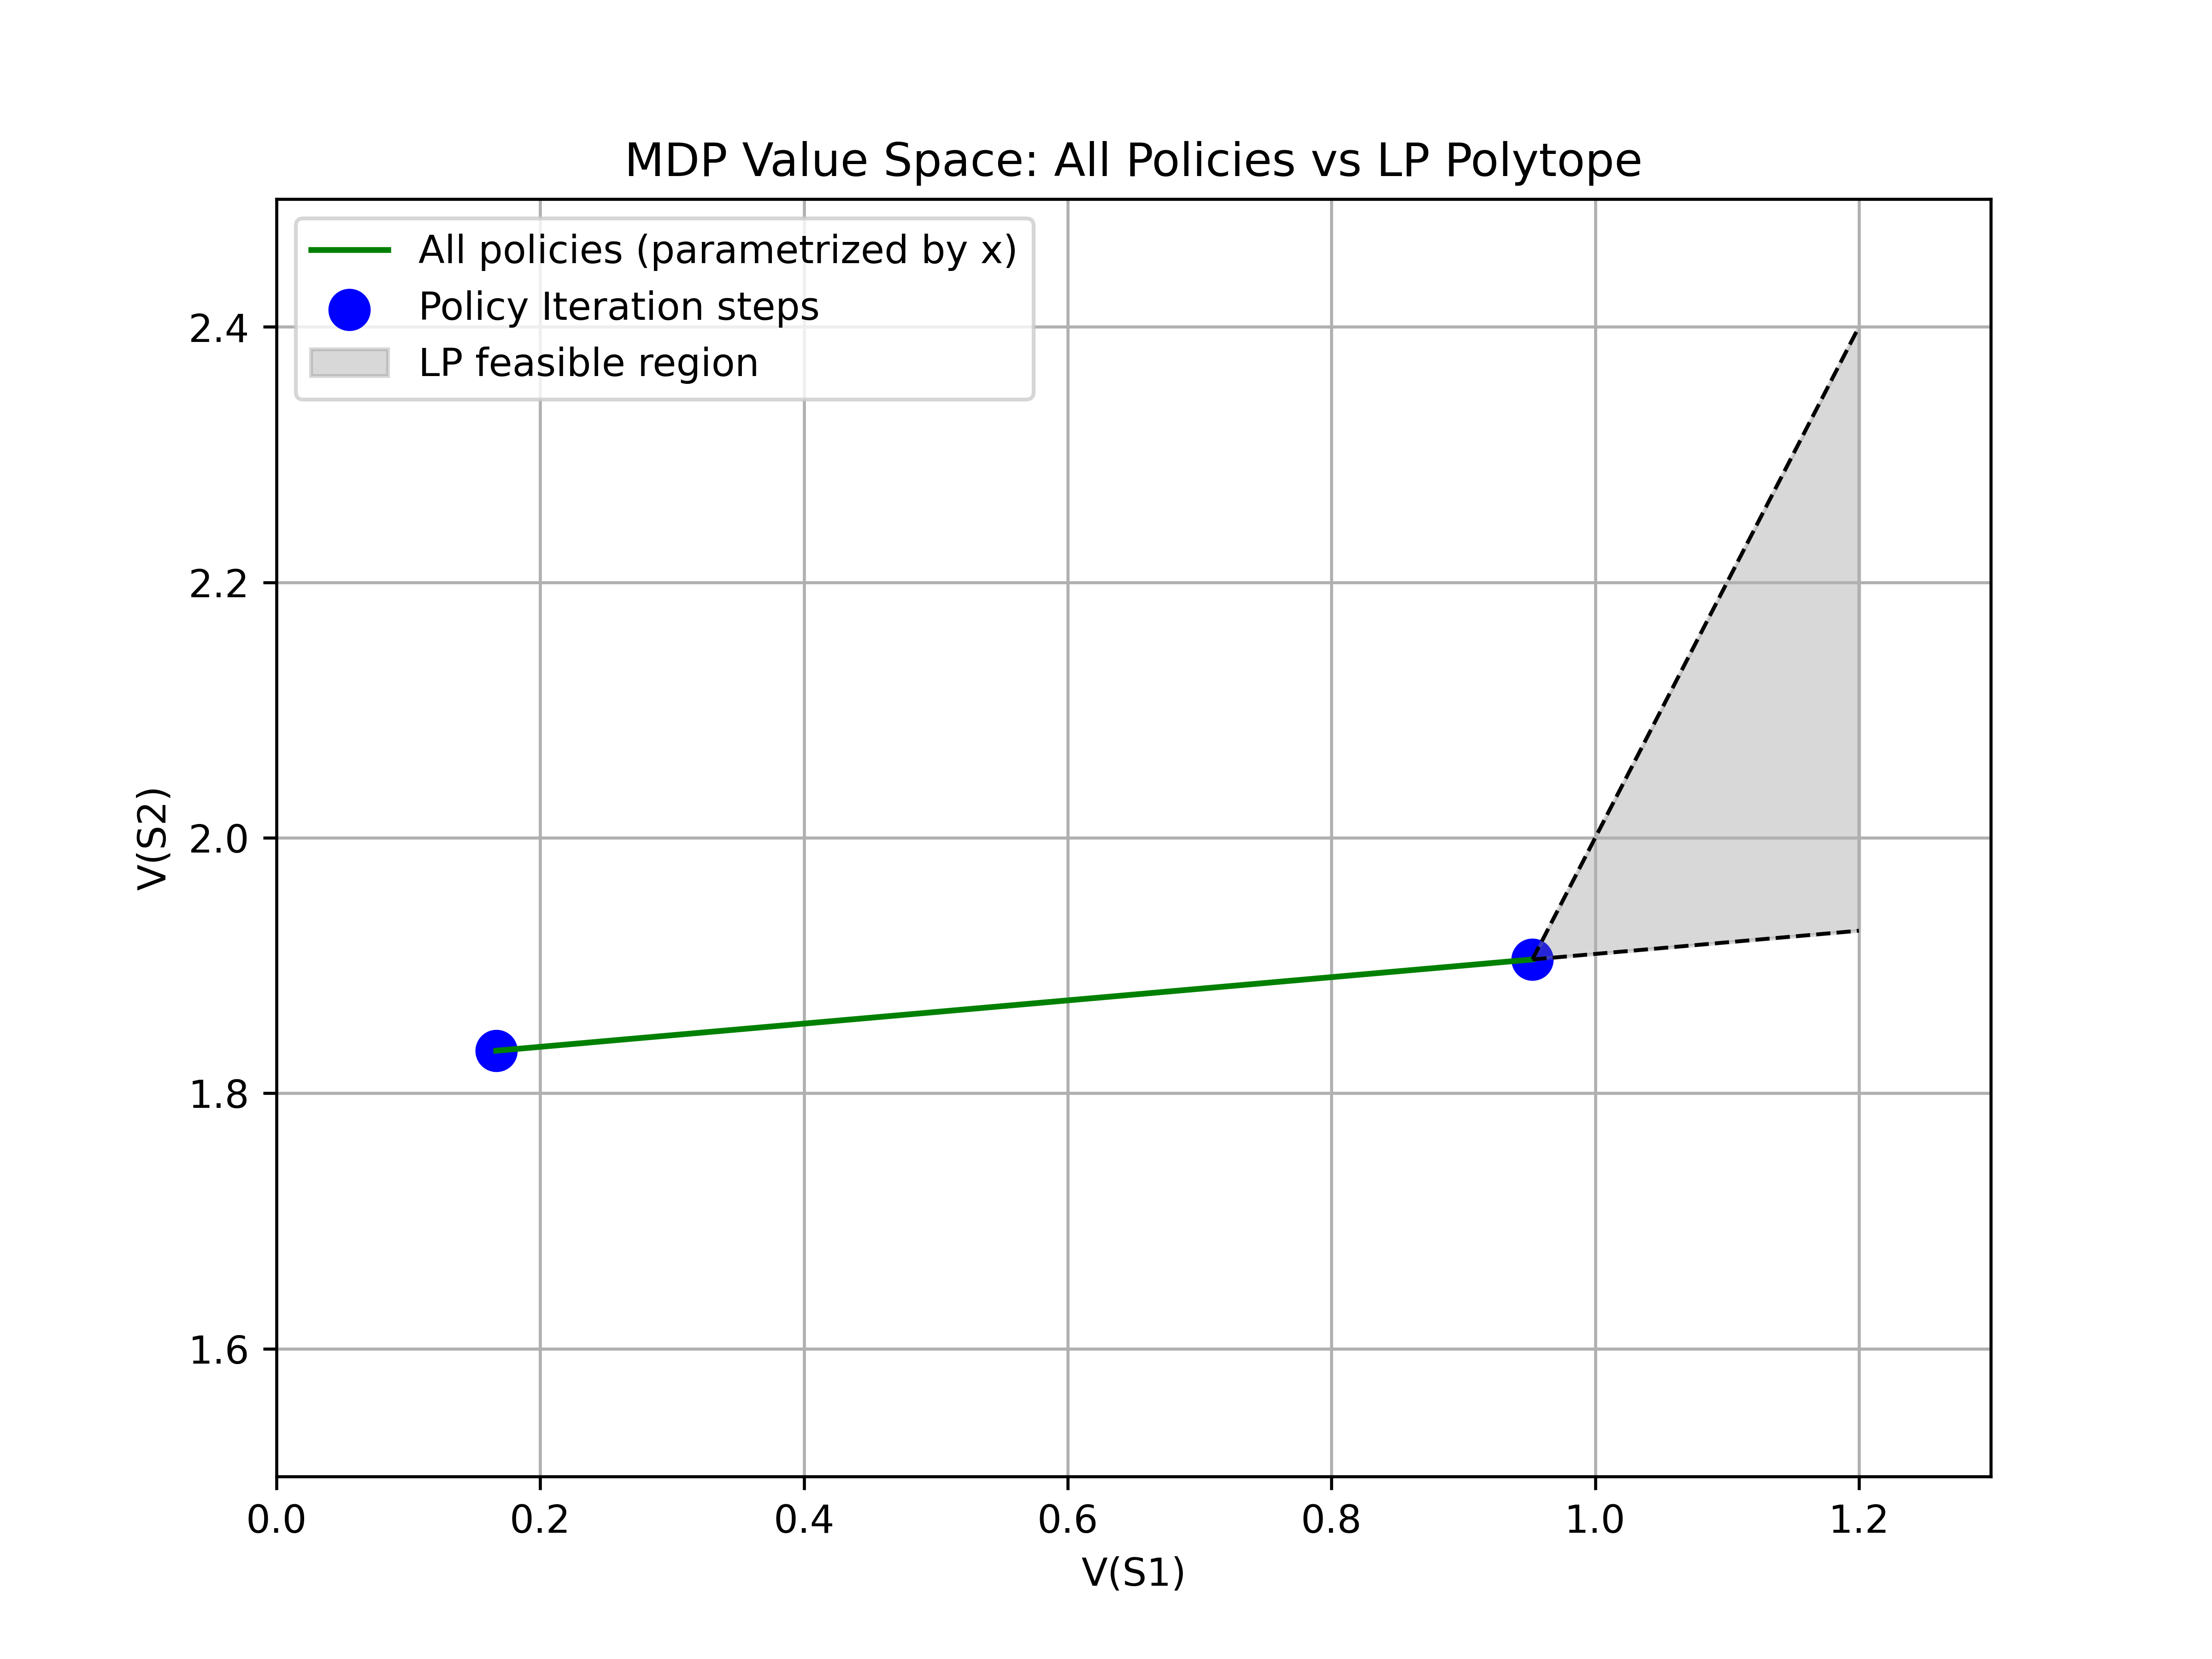
\includegraphics[width=0.8\linewidth]{figures/pi_vs_lp.png}
    \caption{Comparison between LP and PI for the MDP in Figure \ref{fig:vi_vs_pi_example}. We plot the polytope for $z(\state_1), z(\state_2)$ on the same plot of the values $\Value^\policy(\state_1), \Value^\policy(\state_2)$, for every possible policy $\policy$. Note that the polytope intersects with the values only at the optimal policy $\Value^*(\state_1), \Value^*(\state_2)$.}
    \label{fig:pi_vs_lp_plot}
\end{figure}
\end{example}

%
%
%\begin{proposition}
%The solution $v_\ttime(\state)$ of the linear program is the optimal
%value function $\Value_{ttime}(\state)$.
%\end{proposition}
%
%\begin{proof}
%Let $v_\ttime(\state)$ be the solution of the linear program. We
%will show by back ward induction that the values $v_\ttime(\state)$
%are identical to $\Value_\ttime(\state)$ of the Finite-horizon
%Dynamic Programming (Algorithm \ref{Alg:FHDP-DDP}), i.e,
%$v_\ttime(\state)=\Value_\ttime(\state)$.
%
%At $\ttime=\tHorizon$ it holds by the initializations in both cases.
%Consider $\ttime$ and assume that the inductive hypothesis holds for
%$\ttime+1$. This implies that for every action $\action\in\Actions$
%nd state $\state\in\States$, we have
%\[{{\reward_{\ttime}}(\state,\action) + \Value_{\ttime +
%1}^{}({f_{\ttime}}(\state,\action))}=
%{{\reward_{\ttime}}(\state,\action) + v_{\ttime +
%1}^{}({f_{\ttime}}(\state,\action))} .\]
%Therefore we have
%$v_\ttime(\state) \geq \Value_\ttime(\state)$. Since we are
%minimizing over $v_\ttime(\state)$, we have $v_\ttime(\state) \geq
%\Value_\ttime(\state)$.
%\end{proof}

%\end{leftbar}

% \section*{Exercises}
% \input{exercises/MDPs_modified_PI}
% \input{exercises/MDPs_nonlinear_objective}
% \input{exercises/MDPs_Purchasing_with_a_Deadline}


\section{Further Notes}
%Post and Ye \cite{PostY13}.

%Madani et al \cite{MadaniTZ10}.

A rigorous treatment of the relationship between linear programming and MDP planning is given in \cite{puterman2014markov}. A more reinforcement learning specific approach can be found in \cite{FariasR03, desai2009smoothed}.

% Historically, the work of \cite{d1963probabilistic} was the first to formalize a Linear Programming for the discounted return, and \cite{manne1960linear} for the average cost. 

There are works that use a linear programming approach to derive strongly polynomial algorithms. Specifically, for deterministic MDPs we have polynomial time algorithms which are based on linear programming \cite{MadaniTZ10,PostY13}. An important application of the LP approach is in constrained MDPs \cite{altman2021constrained}.